This event option is provided for the user to specify multiple existing
\href{http://peer.berkeley.edu}{PEER} ground
motion files. PEER files contain time-histories in a single degree of freedom; hence, if multi-degree-of-freedom excitation is desired, the user is required to specify each
individual component for every EVENT. The \texttt{Add/Remove} buttons
at the top are to create and remove an event, as
per \Cref{subsec:multiple_existing}. The \texttt{+} and \texttt{-} buttons add and remove
components (see \Cref{fig:PEER_event_panel}). Remove removes all selected components. Each
component in a PEER event can have their own scale factor, which can be assigned a random variable.

\begin{figure}[!htbp]
  \centering {
    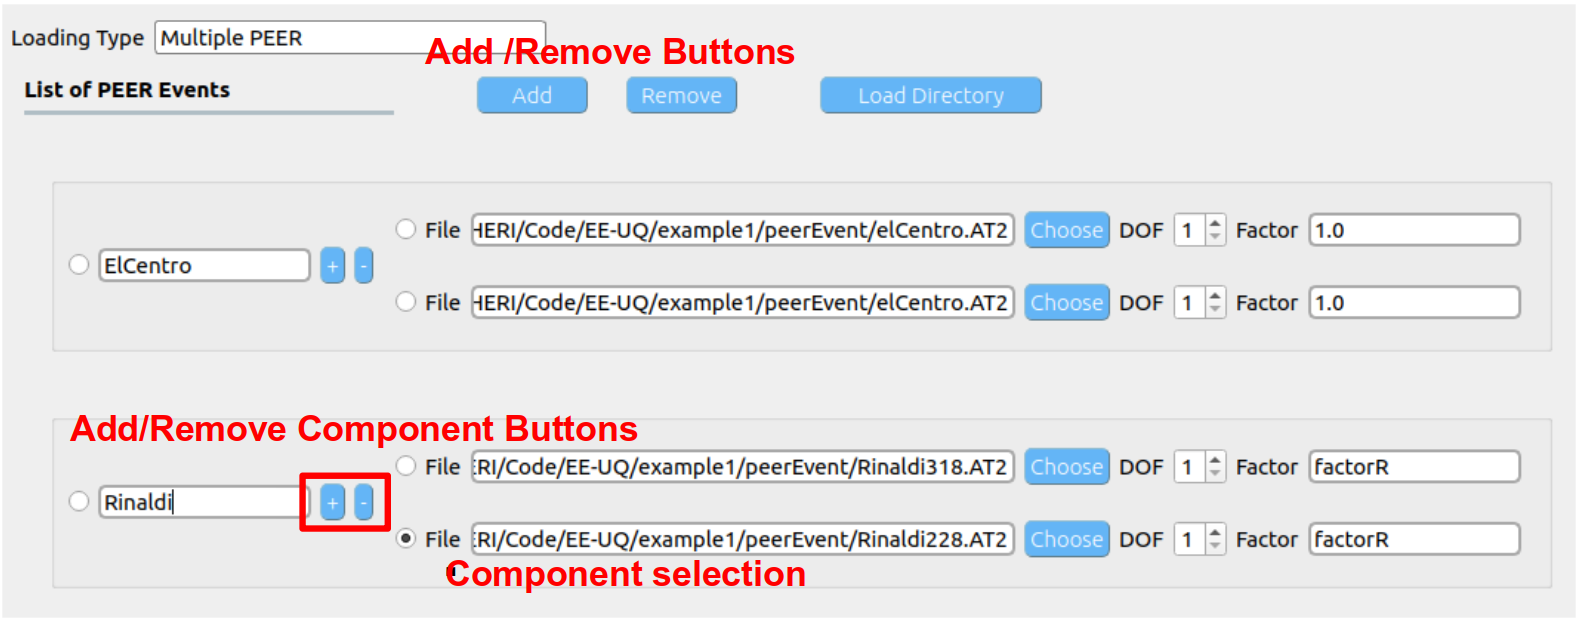
\includegraphics[width=0.8\textwidth]
    {usage/figures/multiplePEER.png} }
  \caption{Multiple PEER Events}
  \label{fig:PEER_event_panel}
\end{figure}

The \txttt{Load Directory} button and the \texttt{Records.txt} file works for PEER events as described in \Cref{subsec:multiple_existing}. The only difference is that PEER files are expected to have an \texttt{.AT2} extension. Only files with that extension shall be specified in the \texttt{Records.txt}.
An example \texttt{Records.txt} file for multiple Peer
events is shown below:

\begin{verbatim}
elCentro.AT2,1.5
Rinaldi228.AT2,2.0
Rinaldi318.AT2,2.0
\end{verbatim}

Random Variables: Random scale factors can be defined by entering a string in the factor field. The variable name entered will appear as a Random Variable in the UQ panel and the user must specify its properties there. If multiple
events are specified, the event itself will be treated as a random
variable, with each event being part of the discrete set of possible
events.